\documentclass[twocolumn]{article}
\usepackage[utf8]{inputenc}
\usepackage[margin=0.5in]{geometry}
\usepackage{graphicx}
\graphicspath{ {./images/} }
\usepackage{hyperref}
\usepackage{xcolor}
\usepackage[T1]{fontenc}
\usepackage{titling}
\usepackage{enumitem}

\setlength{\droptitle}{0em}

\title{Ken Souza Memorial Spaceflight Research Program 2020 Proposal - STAC}
\author{Jasmine Gupta\textsuperscript{1}, Chelsey Fang\textsuperscript{1}, Thomas Devlin\textsuperscript{1}
\\ \textsuperscript{1}Space Technologies at Cal, UC Berkeley, Berkeley, CA USA}
\date{June 2020}

\begin{document}

\maketitle

\section{Introduction}
The increasing prevalence of antibiotic resistance among pathogenic bacteria is a problem that threatens global human health. In 2013, the CDC declared that the human race is in the “post-antibiotic era” and the World Health Organization has also warned that the crisis has become dire.\textsuperscript{1} The CDC estimates that it costs the American healthcare system 20 billion dollars per year in direct costs, with indirect lost productivity costs of up to 35 billion dollars.\textsuperscript{2} Consequently, understanding how microbes obtain resistance to antibiotics will help us reverse-engineer solutions to the problem. 

The challenging field of human space flight contends with many physiological and biological challenges. Some are well documented, such as muscle atrophy due to lack of gravity, others, like the decrease in antibiotic efficacy are less well understood.\textsuperscript{3,4} Microorganisms have the ability to respond almost immediately to environmental changes.\textsuperscript{5} This ability allows them to adapt and survive in extreme environments, such as microgravity. Literature has discussed the upregulation of genes involved in “starvation response, acid stress, osmotic stress, oxidative stress, biofilm formation, curli biosynthesis and lipid biosynthesis” upon exposure to microgravity\textsuperscript{5}. Because the genes for biofilm formation are upregulated, there is greater biofilm production, creating thicker and more robust biofilms.\textsuperscript{5} These biofilms prevent antibiotics from working effectively or even at all. As such, there is higher resistance to antibiotics in microgravity. The phenomena of increased resistance has been shown in a previous study aboard the ISS using both E. coli and the antibiotic Gentamicin.\textsuperscript{6}

We aim to utilize the unique opportunity presented by Blue Origin’s New Shepard flight to test the effects of short term exposure to microgravity in tandem with long-term simulated microgravity experiments on the ground to understand how exposure to microgravity affects bacterial resistance to antibiotics. We will expand upon previous studies and focus on how changes in gene expression correspond to changes in resistance.

\section{Hypothesis}
The combined stress of launch into spaceflight and subsequent microgravity environment activates a change in bacterial gene expression that renders them less susceptible to the antibiotic Gentamicin. Further exploration of differential gene expression will elucidate general mechanisms that result in antibiotic resistance. 

\section{Research Objectives}
\begin{enumerate}
    \item To utilize microgravity to understand the development of evolutionary resistance to antibiotics.
    \item To understand the effects of microgravity on the clinical microbiome as well as on bacterial transcriptomics and physiology.
    \item To demonstrate the utility of commercial spaceflight for proof-of-concept biological experiments.
\end{enumerate}

\section{Experimental Design}

When bacteria is in need of a change in protein composition due to an outside stress, RNA polymerases are recruited to create RNA templates of the corresponding sections of the DNA genome. These templates are made into the desired proteins by ribosomes. This ability to control protein production allows cells to adapt and survive in extreme environments such as microgravity. By reading the RNA that is present in a culture sample, one can see which genes are in greater or lesser demand, and therefore one can tell how the cell is adapting to environmental changes.

\begin{figure}[h]
    \centering
    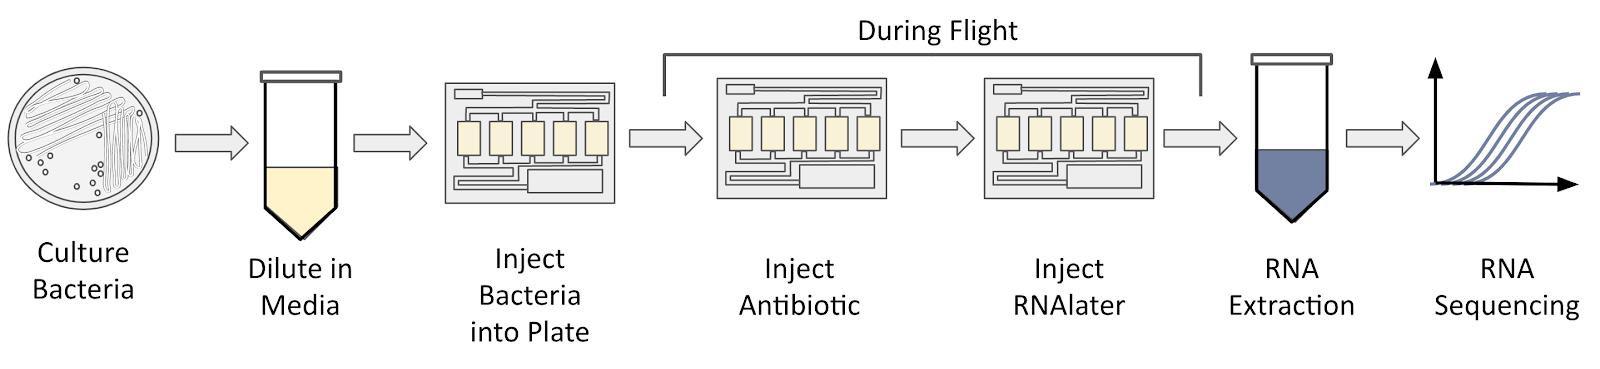
\includegraphics[scale = 0.22]{images/sequence1.png}
    \caption{Basic Experiment Workflow}
    \label{fig:my_label}
\end{figure}

The general design of our microgravity experiment consists of five parts (see Fig 1): 

\begin{enumerate}
    \item Before delivery of the payload, we will inoculate E. coli bacteria into LB media at a concentration that will ensure the bacteria will be in the log phase of growth during flight. We plan to determine this concentration through experiments to characterize the growth curve of E. coli at the maintained temperature of our payload. This ensures the maximum amount of change in gene expression and therefore maximizes the data significance. Addressing concerns regarding the inflight culture of E. coli, it is a low-maintenance bacteria and easily replicates once provided solely with media, therefore, once in LB, it will continue to grow until saturation or RNAlater (RNA fixative) injection in our case. We plan to use the Pad Load option to improve the viability of our colony.
    
    \item We will expose the variable plates of E. coli to the antibiotic Gentamicin at various time points, shown in Fig 2.\\
    \vspace{-5mm}
    \begin{figure}[h]
        \centering
        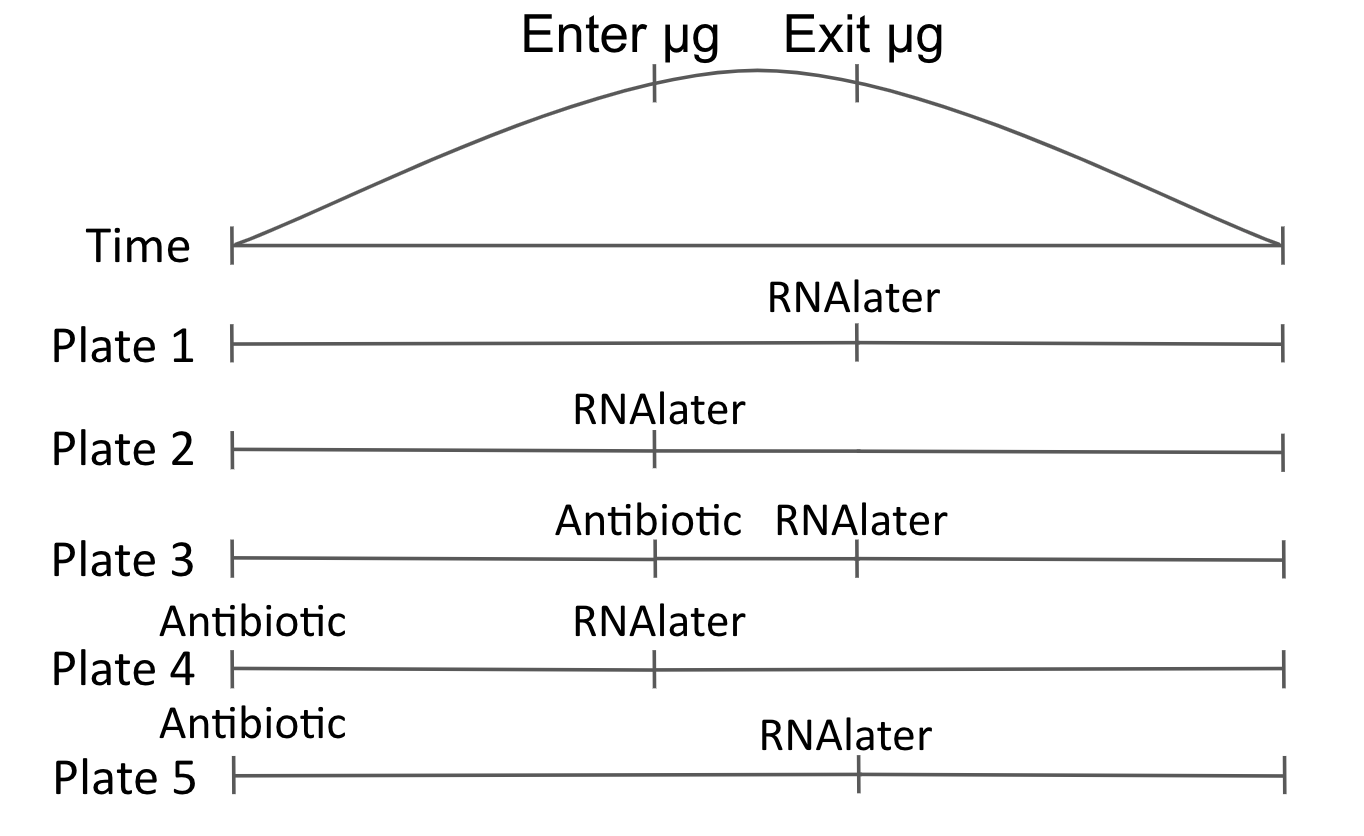
\includegraphics[scale = 0.28]{images/timeline2.png}
        \caption{Timeline for Injection of Antibiotic and RNAlater during flight}
        \label{fig:my_label}
    \end{figure}
    
    \item We will arrest bacterial growth and preserve the RNA expression profile of the bacteria through fixation with RNALater (see Fig 2). 
    RNAlater is a fixative which “freezes” gene expression by stabilizing RNA transcripts in a solution. We have successfully made RNALater in the lab and have used it to preserve extracted RNA for 24 hours at room temperature and long term at -20\textsuperscript{o}C. This allows us to analyze the gene expression of E. coli in microgravity after the payload has returned to earth. Our payload will be delivered to our group on dry ice (-80\textsuperscript{o}C) within 24 hours of return for analysis.
    
    \item Concurrently, the same procedure will be executed on the ground in order to differentiate between RNA composition changes that occur normally, versus those that occur as a result of our experiment. We will perform an RNA extraction on both the ground sample and payload, and will send our results for sequencing to the Berkeley Quantitative Biosciences genomic sequencing facility. We have honed our procedure for RNA extraction through multiple experiments and have consistently obtained quality RNA. We have checked its quality through gel electrophoresis and have not seen any degradation or contamination. 
    \item We will examine our RNA sequencing results to observe the differences in gene expression between the bacteria from the payload and the bacteria from the control experiment on the ground. 
\end{enumerate}

As shown in Fig 2, we will have 5 plates in the payload, allowing us to implement different conditions with each plate containing 5 replicates. For our first plate, we aim to have a control to see the overall differential gene expression over the entire course of the flight. Plate 2 fixes the cells right after we exit microgravity conditions while Plate 3 fixes them right before entering microgravity. With these 3 controls we are able to isolate the changes in gene expression at each portion of the flight and the specific responses to solely hypergravity or microgravity by comparing them with results from the ground experiment. This will allow us to determine what changes are specifically due to the added stress of the antibiotic in each specific condition. Plates 4 and 5 are our test conditions, with the antibiotic injected at the beginning of the condition in question and RNAlater injected at the end of said condition.  


\section{Engineering}
The main engineering challenge of our project focuses on the design and automation of a flight-ready payload for parabolic launch on the New Shepard Rocket. At the time of our proposal last year, our payload’s flight hardware was in early stages of development. Feedback we received after the proposal noted that, “the flight hardware design appears prohibitively difficult to achieve in a 2U payload format”. Since the time of that proposal we have developed and prototyped that hardware extensively and made vast improvements on our old designs.
\begin{figure}[h]
    \centering
    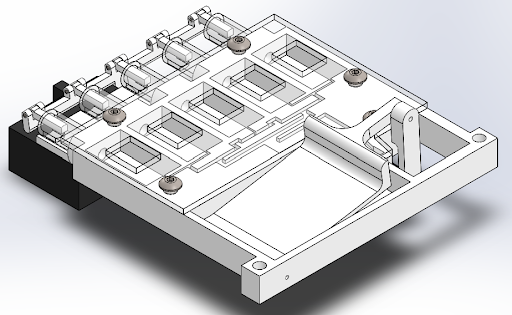
\includegraphics[scale = 0.40]{images/plate.png}
    \caption{A single treatment plate}
    \label{fig:my_label}
\end{figure}
One concern was the weight limit. Our current mass budget takes all systems and components into account and comes in at 478 g, which is under the 500 g limit. This budget is based not only off of nominal masses found in documentation, but also empirically verified assembly masses. Another issue was the difficulty of implementing a precise injection system. As our experiment requires injection of two fluids, our solution has two parts. For RNALater to be effective, we inject a 1:1 ratio of the reagent to E. Coli medium. This means that we can err on the side of injecting extra reagent, which we do. In the case of the antibiotic, precision is necessary. For this reason we have iterated over several injection methods. Our current method for antibiotic injection, which takes advantage of precise micropipetting, has been tested and has less than 2.5\% error. Because consistency is a key factor, we have developed and tested loading procedures for both fluids.

We also have fully developed electronics and software ready for testing. We have custom printed circuit boards which will soon have components mounted for testing. We also have software written to run on an Arduino processor and have conducted preliminary tests using a flight simulator. As noted in the feedback we received, the growth stage of the \emph{E. coli} at launch is very important. A temperature regulation system will maintain a constant temperature within an acceptable range for growth. Given a constant temperature, we can create a growth curve to determine the cell density of E. coli necessary to achieve log phase growth during microgravity and dilute our inoculation accordingly. This timing ensures that cells will be growing exponentially in microgravity, providing maximum RNA expression. Including this heating system, we have created a power budget totalling 2.38 W, and expect to be able to run off of the USB power supplied by Blue Origin.
\vspace{-7mm}
\begin{figure}[h]
    \centering
    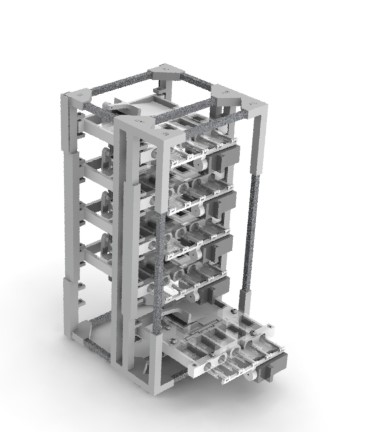
\includegraphics[scale = 0.6]{images/Chassis.JPG}
    \caption{Overall chassis assembly}
    \label{fig:my_label}
\end{figure}

Under the parameters set by Blue Origin, we have constructed a chassis whose dimensions lie within the 2U requirement. Additionally, due to the biological aspect of this experiment, two levels of containment are required. The first layer of containment is a layer of BreatheEasy, a gas-permeable membrane to seal the plate and restrict liquid flow. For the second layer of containment, there are removable sheets that will slide and lock into each side of the chassis during the experiment and have the ability to release after the experiment in order to collect the samples. Considering the experimental plates need to be easily accessible before and after the experiment for analysis, we have designed the chassis to structurally support each plate and allow for easy access, yet strong connections. Furthermore, we have designed the chassis with carbon fiber supports to give us high stiffness and low weight to help accommodate the 500 g weight limit.

\section{Public Engagement}
\begin{figure}[h]
    \centering
    
\includegraphics[scale = 0.28]{images/outreach.jpg}
    \caption{Outreach Efforts}
    \label{fig:my_label}
\end{figure}
Another focus of our team is to increase the accessibility of space and inspire STEM education in the East Bay community. This team is a part of Space Technologies at Cal (STAC), a group of 60 passionate UC Berkeley students who are working on a range of technologies aimed at making strides in space research. We continually engage our peers at UC Berkeley and the community at large, building on our past experience and applying it to the public engagement aspect of this payload. For the past few years, we have invited high school students to collaborate with us during summers to get hands on experience designing and building technology for space applications. We have plans to further connect with local high schools to talk about current space news as well as collaborate on educational projects such as HAB launches. The past two years, STAC has hosted a Space Tech Symposium, inviting industry members, academia, and VC’s in the Bay Area to speak on panels and create an event that brings people interested in Space together. A successful launch would help spur interest in the event and help inspire other groups to learn and experiment in Space. We also plan to continue submitting our finalized research results to a variety of conferences (like ASGSR, ASM, etc.), writing publically available blog posts on Medium, and promoting external education student outreach.

\section{Conclusion}
The opportunity to conduct cheaper, more inexpensive microgravity experiments with Blue Origin represents a paradigm shift in how we can use spaceflight to tackle conventional biological questions. The proposed project demonstrates the ability for a student-led research initiative (STAC) to tackle a pressing biomedical problem: the issue of global antibiotic resistance.  

\section{Current Relationships and Collaborators}
\begin{itemize}
    \item Steve Ruzin: UC Berkeley Faculty Mentor, Director of the CNR Biological Imaging Facility
    \item Gian Garriga: UC Berkeley Professor of Molecular and Cell Biology
    \item Antonio Ricco: Chief Technologist at NASA Ames for Small Payloads
    \item Luis Zea: Assistant Research Professor at University of Colorado, Boulder with Bioserve Technologies
\end{itemize}
\vspace{-4mm}
\section{References (links)}
\vspace{-2mm}
\begin{enumerate}[nosep]
    \item \textcolor{blue}{\href{https://www.ncbi.nlm.nih.gov/pmc/articles/PMC4165128/}{www.ncbi.nlm.nih.gov    (1)}}
    \item \textcolor{blue}{\href{https://www.cdc.gov/media/releases/2013/p0916-untreatable.html}{www.cdc.gov}}
    \item \textcolor{blue}{\href{https://www.nasa.gov/pdf/64249main_ffs_factsheets_hbp_atrophy.pdf}{www.nasa.gov}}
    \item \textcolor{blue}{\href{https://www.sciencedirect.com/science/article/abs/pii/S0167779906000266}{www.sciencedirect.com}}
    \item \textcolor{blue}{\href{https://www.ncbi.nlm.nih.gov/pmc/articles/PMC3589462/}{www.ncbi.nlm.hib.gov    (2)}}
    \item \textcolor{blue}{\href{https://www.colorado.edu/faculty/zea-luis/sites/default/files/attached-files/zea_-_thesis_-_published.pdf}{www.colorado.edu/faculty/zea-luis}}
\end{enumerate}


\end{document}
